\documentclass[a4paper, 11pt, oneside]{article} % A4 paper size, default 11pt font size and oneside for equal margins

\newcommand{\plogo}{\fbox{$\mathcal{PL}$}} % Generic dummy publisher logo

\usepackage[utf8]{inputenc} % Required for inputting international characters
\usepackage[T1]{fontenc} % Output font encoding for international characters
\usepackage{fouriernc} % Use the New Century Schoolbook font
\usepackage{titlesec}
\usepackage{url}
\def\UrlBreaks{\do\/\do-}
\usepackage{breakurl}
\usepackage[breaklinks]{hyperref}
\usepackage{float}
\usepackage{etoolbox}
\patchcmd{\thebibliography}{\section*}{\section}{}{}
\titleformat{\chapter}[block]
  {\normalfont\huge\bfseries}{\thechapter}{20pt}{}
\titlespacing*{\chapter}
  {0pt}{20pt}{20pt}

\setcounter{tocdepth}{5}
\setcounter{secnumdepth}{5}

\usepackage[utf8]{inputenc}
\usepackage[english]{babel}
 
\setlength{\parindent}{4em}
\setlength{\parskip}{1em}
\renewcommand{\baselinestretch}{1.5}


\usepackage{hyperref}
\hypersetup{
    colorlinks=true,
    linkcolor=blue,
    filecolor=magenta,      
    urlcolor=cyan,
}

\usepackage{graphicx}

\usepackage{textcomp}


%----------------------------------------------------------------------------------------
%	TITLE PAGE
%----------------------------------------------------------------------------------------

\begin{document} 




\begin{titlepage} % Suppresses headers and footers on the title page




	\centering % Centre everything on the title page
	
	\scshape % Use small caps for all text on the title page
	
	\vspace{0\baselineskip} % White space at the top of the page
	\vspace{0.5\baselineskip} % Whitespace below the editor list
	
	{\scshape\Large Cairo University\\ Faculty of Engineering\\Systems And Biomedical Engineering\\} % Editor affiliation

	%------------------------------------------------
	%	Title
	%------------------------------------------------
	
	\rule{\textwidth}{1.6pt}\vspace*{-\baselineskip}\vspace*{2pt} % Thick horizontal rule
	\rule{\textwidth}{0.4pt} % Thin horizontal rule
	
	\vspace{0.75\baselineskip} % Whitespace above the title
	
	{\LARGE THORACIC   SURGERY\\ SURVIVAL PROPOSAL\\} % Title
	
	\vspace{0.75\baselineskip} % Whitespace below the title
	
	\rule{\textwidth}{0.4pt}\vspace*{-\baselineskip}\vspace{3.2pt} % Thin horizontal rule
	\rule{\textwidth}{1.6pt} % Thick horizontal rule
	
	\vspace{0\baselineskip} % Whitespace after the title block

	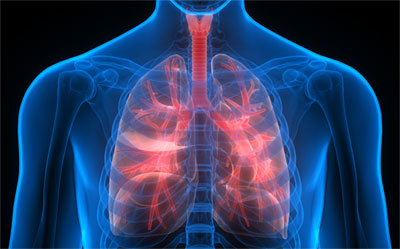
\includegraphics[width=12cm, height=5 cm]{figures/Thoracic-Anesthesiology}
	
	%------------------------------------------------
	%	Editor(s)
	%------------------------------------------------
	
	Group Number : 2\\
         \vspace{1\baselineskip} 
        Group Members :
	
	\vspace{0.5\baselineskip} % Whitespace before the editors
  
	
	{\scshape\Large Asmaa Mahmoud Mahmoud\\ Alaa Gamal Abdelaziz\\Salma Mohamed Zakaria\\Marwa Adel Youssef\\} % Editor list
	
	
	
	\vfill % Whitespace between editor names and publisher logo
	
	%------------------------------------------------
	%	Publisher
	%------------------------------------------------
	

	
	\vspace{0.3\baselineskip} % Whitespace under the publisher logo
	
	%2019 % Publication year
	
	

\end{titlepage}

%----------------------------------------------------------------------------------------
\section{Project background and motivation}

We have chosen Thoracic surgery as its evolving and surgeons have major collaborative roles in management of lung cancer, respiratory infections, chest trauma, pediatric respiratory disorders and end-stage respiratory. Today, lung cancer is the most frequent indication for thoracic surgery.
Thoracic Surgeries focuses on the chest organs, including the esophegus , trachea , pleura , chest wall, diaphragm, heart, and lungs. Technological advances have increased the safety and availability of these complex surgical procedures. Lung cancer surgeries and anti-reflex surgeries save and improve lives around the world.
The most common diseases requiring thoracic surgery include lung cancer (its rate of survival is very low among women and men) , chest trauma (require urgent thoracic surgery), esophageal cancer,(its rate is rising slowly recently) emphysema, and lung transplantation.
So in conclusion we chose this project because we are hopeful that our model will be useful to detect the patients who are at risk after surgery by importing their symptoms in our model which we will be using the data from former patients’ information in.\cite{encyclopedia} 
\newpage
\section{Objectives of project }
\begin{enumerate}

\item Learning statistics which is mathematical study of data as you cannot do statistics without having data and it will be done by using statistical model which is a model for the data that is used either to infer something about the relationships within the data or to create a model that is able to predict future values. \cite{towardsdatascience1} 
\item Making statistical models which are designed for inference about the relationships between variables.
\item Learning Machine learning which has a purpose of obtaining a model that can make repeatable predictions. 
\item Learning the three methods of the machine learning which are:
\begin{itemize}
\item Naive Bayes (NB) Classier (or Gaussian NB Classifier).
\item K-nearest neighbors (KNN) model.
\item Logistic regression.
\end{itemize}
\item Learning how to make Data Visualization.

\end{enumerate}
\section{Data Set Information:} 

The data was collected retrospectively at Wroclaw Thoracic Surgery Centre for patients who underwent major lung resections for primary lung cancer in the years 2007 \& 2011. The Centre is associated with the Department of Thoracic Surgery of the Medical University of Wroclaw and Lower-Silesian Centre for Pulmonary Diseases, Poland, while the research database constitutes a part of the National Lung Cancer Registry, administered by the Institute of Tuberculosis and Pulmonary Diseases in Warsaw, Poland.\cite{archive} 
\subsection{Attribute Information:} 
\begin{enumerate} 
\item DGN: Diagnosis -specific combination of ICD-10 codes for primary and secondary as well multiple tumours if any (DGN3, DGN2, DGN4, DGN6, DGN5, DGN8, DGN1)
ICD-10 codes are alphanumeric codes used by doctors, health insurance companies, and public health agencies across the world to represent diagnoses. Every disease, disorder, injury, infection, and symptom has its own ICD-10 code. 
\item ForcedVitalCapacity : is the total amount of air exhaled during the Forced Expiatory Volume test. FVC (numeric) 
\item ForcedExpiratoryVolume1: Volume that has been exhaled at the end of the first second of forced expiration - FEV1 (numeric)\\
Diagnose obstructive lung diseases such as asthma and chronic obstructive pulmonary disease (COPD). A person who has asthma or Chronic Obstructive Pulmonary Disease has a lower FEV1 result than a healthy person.
\begin{itemize}
\item See how well medicines used to improve breathing are working.
\item Check if lung disease is getting worse. Decreases in the FEV1 value may mean the lung disease is getting worse.
\end{itemize}

\item PerformanceStatus: - Zubrod scale (PRZ2,PRZ1,PRZ0)\\
Zubrod score runs from 0 to 5, with 0 denoting perfect health and 5 death: Its advantage lies in its simplicity.
\begin{itemize}
\item 0 – Asymptomatic (Fully active, able to carry on all predisease activities without restriction)
\item 1 – Symptomatic but completely ambulatory (Restricted in physically strenuous activity but ambulatory and able to carry out work of a light or sedentary nature. For example, light housework, office work)
\item  2– Symptomatic, <50\% in bed during the day (Ambulatory and capable of all self care but unable to carry out any work activities. Up and about more than 50\% of waking hours)
\item 3 – Symptomatic, >50\% in bed, but not bedbound (Capable of only limited self-care, confined to bed or chair 50\% or more of waking hours)
\item 4– Bedbound (Completely disabled. Cannot carry on any self-care. Totally confined to bed or chair)
\item 5 – Death
\end{itemize}
\item  PainBS: Pain before surgery (T,F)
\item HaemoptysisBS: Haemoptysis before surgery (T,F)
\begin{itemize}
\item {Hemoptysis:}
is the coughing up of blood or blood-stained mucus from the bronchi, larynx, trachea, or lungs
\end{itemize}
\item  DyspnoeaBS: Dyspnoea before surgery (T,F)
\begin{itemize}
\item{dyspnea :}
is the feeling that one cannot breathe well enough. (Shortness of breath)
\end{itemize}
\item  CoughBS: Cough before surgery (T,F)
\item WeaknessBS: Weakness before surgery (T,F)
\item SizeOfTumer: T(Tumer) in clinical TNM - size of the original tumour, from OC11(smallest) to OC14(largest)  (OC11,OC14,OC12,OC13)
\begin{itemize}
\item {The TNM Classification of Malignant Tumors (TNM):}
is a globally recognised standard for classifying the extent of spread of cancer.
\end{itemize}
\item Type2Diabetes: Type 2 DM - diabetes mellitus (T,F)
\item HeartAttack6M: MI up to 6 months (T,F)
\begin{itemize}
\item{Myocardial infarction (MI):}
 also known as a heart attack has happened in the last 6 months
\end{itemize}
\item PeripheralArterialDiseases: PAD - peripheral arterial diseases (T,F)
\begin{itemize}
\item {Peripheral arterial disease}
is a common circulatory problem in which narrowed arteries reduce blood flow to your limbs. 
\end{itemize}
\item Smoking (T,F)
\item  Asthma (T,F)
\begin{itemize}
\item {Asthma}
is a condition in which your airways narrow and swell and produce extra mucus. This can make breathing difficult and trigger coughing, wheezing and shortness of breath.
\end{itemize}
\item Age: Age at surgery (numeric)
\item Risk1Y: 1 year survival period - (T)rue value if died (T,F)
\end{enumerate}
\subsection {Class Distribution:}
the class value (Risk1Y) is binary valued.
\begin{itemize}
\item Risk1Y Value: Number of Instances:
\begin{itemize}
\item {T $\leftarrow$ 70}
\item {F $\leftarrow$ 400}
\end{itemize}
\end{itemize}
\newpage
\subsection {Summary Statistics:}
\begin{enumerate}
\item{Binary Attributes Distribution:}
\begin{itemize}
\item{PainBS Value: Number of Instances:}
\begin{itemize}
\item T $\leftarrow$ 31
\item F $\leftarrow$ 439
\end{itemize}
\item {HaemoptysisBS Value: Number of Instances:}
\begin{itemize}
\item T $\leftarrow$ 68
\item F$\leftarrow$402
\end{itemize}
\item{DyspnoeaBS Value: Number of Instances:}
\begin{itemize}
\item T$\leftarrow$31
\item F $\leftarrow$439
\end{itemize}
\item{CoughBS Value: Number of Instances:}
\begin{itemize}
\item T $\leftarrow$323
\item F $\leftarrow$147
\end{itemize}
\item{WeaknessBS Value: Number of Instances:}
\begin{itemize}
\item T $\leftarrow$ 78
\item F $\leftarrow$ 392
\end{itemize}
\item{Type2Diabetes Value: Number of Instances:}
\begin{itemize}
\item T$\leftarrow$35
\item F $\leftarrow$ 435
\end{itemize}
\item{HeartAttack6M Value: Number of Instances:}
\begin{itemize}
\item T $\leftarrow$ 2
\item F $\leftarrow$468
\end{itemize}
\item{PeripheralArterialDiseases Value: Number of Instances:}
\begin{itemize}
\item T $\leftarrow$ 8
\item F $\leftarrow$ 462
\end{itemize}
\item{Smoking Value: Number of Instances:}
\begin{itemize}
\item T $\leftarrow$386
\item F $\leftarrow$84
\end{itemize}
\item{Asthma Value: Number of Instances:}
\begin{itemize}
\item T $\leftarrow$ 368
\item F $\leftarrow$ 2
\end{itemize}
\end{itemize}
\item {Nominal Attributes Distribution:}
\begin{itemize}
\item{DGN Value: Number of Instances:}
\begin{itemize}
\item DGN3 $\leftarrow$ 349 
\item DGN2 $\leftarrow$ 52 
\item DGN4 $\leftarrow$ 47
\item DGN6 $\leftarrow$ 4
\item DGN5 $\leftarrow$ 15
\item DGN8 $\leftarrow$ 2
\item DGN1$\leftarrow$1
\end{itemize}
\item{PerformanceStatus Value: Number of Instances:}
\begin{itemize}
\item PRZ2 $\leftarrow$ 27
\item PRZ1 $\leftarrow$ 313
\item PRZ0 $\leftarrow$ 130
\end{itemize}

\item{SizeOfTumer Value: Number of Instances:}
\begin{itemize}
\item OC11 $\leftarrow$ 177
\item OC14 $\leftarrow$ 17
\item OC12 $\leftarrow$ 257
\item OC13 $\leftarrow$ 19
\end{itemize}
\end{itemize}
\item {Numeric Attributes Statistics:}\\\\
\begin{tabular}{ |p{4.5cm}||p{2cm}|p{2cm}|p{2cm}| p{2cm}| }
 \hline
 Numeric Attributes&Min& Max&Mean&STD\\
 \hline
ForcedVitalCapacity   & 1.4    &6.3&  3.3 &0.9 \\
ForcedExpiratoryVolume1 &  0.96  & 86.3   &4.6 &11.8\\
 Age &21 & 87&  52.5 & 8.7\\
 \hline
\end{tabular}

\end{enumerate}

\section {Pre-processing of Data}
In recent year, the difficulty for creating model increasing explosively as the data to be analyzed growing. When the attempt is classifying or creating a model for a specified problem, the various technique could be used, but dealing with problems contain a high number of features is a very challengeable task. So we will be focusing on the analyzing and selecting the data using statistical methods before creating the model.

In our data we have three scale variables and thirteen nominal variables, So we need to determine the correlation between the scale and nominal variables and the one-year status.\cite{researchgate} 

We will use statistical tests to analyze and visualize the Thoracic Surgery Data. We will use two types of relations. The ANOVA test \cite{analyticsvidhya1} between the one-year status and scale variables while the chi-square\cite{mathsisfun}  between one-year status and the nominal variables. From the 16 variables, the related variables with the one year-status will be the variables which we will use to create our model. Therefore, we could create a model with less number of variables by understanding and visualizing the dataset. 

However we won’t do any data imputation in our statistical model because our dataset is complete and doesn’t have any missing values in them.

\section{Exploratory data analysis (EDA)}
Exploratory data analysis depends on visualization of data by using \textbf { R-Language} libraries  as \textbf {ggplot}.\\
From point 4 after using correlation, we mentioned that we have two tables one between the one-year status and scale variables while the other between one-year status and the nominal variables so we will use statistical tests to analyze and visualize the one-year status that depend on variables known from point 4.\cite{datacamp} 

\section{Methodology}

\subsection{Naive Bayes} 
 Naive Bayes is a classification algorithm for binary (two-class) and multi-class classification problems. The technique is easiest to understand when described using binary or categorical input values\\.
It is called naive Bayes or idiot Bayes because the calculation of the probabilities for each hypothesis are simplified to make their calculation tractable. Rather than attempting to calculate the values of each attribute value $P(d1, d2, d3|h)$ , they are assumed to be conditionally independent given the target value and calculated as $P(d1|h)P(d2|H)$ and so on.\\
This is a very strong assumption that is most unlikely in real data, i.e. that the attributes do not interact. Nevertheless, the approach performs surprisingly well on data where this assumption does not hold.\cite{analyticsvidhya2} \\
Bayes’ Theorem is stated as: 
\\
$P(h|d) = \frac { (P(d|h)P(h)}{P(d)}$\\
Where\\
\begin{itemize}
\item$P(h|d)$ is the probability of hypothesis h given the data d. This is called the posterior probability.
\item$P(d|h)$ is the probability of data d given that the hypothesis h was true.
\item P(h) is the probability of hypothesis h being true (regardless of the data). This is called the prior probability of h.
\item P(d) is the probability of the data (regardless of the hypothesis).
\end{itemize}
You can see that we are interested in calculating the posterior probability of $P(h|d)$ from the prior probability P(h) with P(d) and $P(d|h)$.\\

Gaussian Naive Bayes\\
Naive Bayes can be extended to real-valued attributes, most commonly by assuming a Gaussian distribution.
This extension of naive Bayes is called Gaussian Naive Bayes. Other functions can be used to estimate the distribution of the data, but the Gaussian (or Normal distribution) is the easiest to work with because you only need to estimate the mean and the standard deviation from your training data.\\

Advantages of Naive Bayes:
\begin{enumerate}
\item When assumption of independent predictors holds true, a Naive Bayes classifier performs better as compared to other models.

\item Naive Bayes requires a small amount of training data to estimate the test data. So, the training period is less.

\item Naive Bayes is also easy to implement.
\end{enumerate}
\newpage



\subsection{Logistic regression}   
Logistic regression is a technique borrowed by machine learning from the field of statistics.\\
It is the go-to method for binary classification problems (problems with two class values) in our case it’s whether the patient died after one year or not(0,1).\\
We can call a Logistic Regression a Linear Regression model but the Logistic Regression uses a more complex cost function, this cost function can be defined as the ‘Sigmoid function’ or also known as the ‘logistic function’ instead of a linear function.\cite{machinelearningmastery} \\


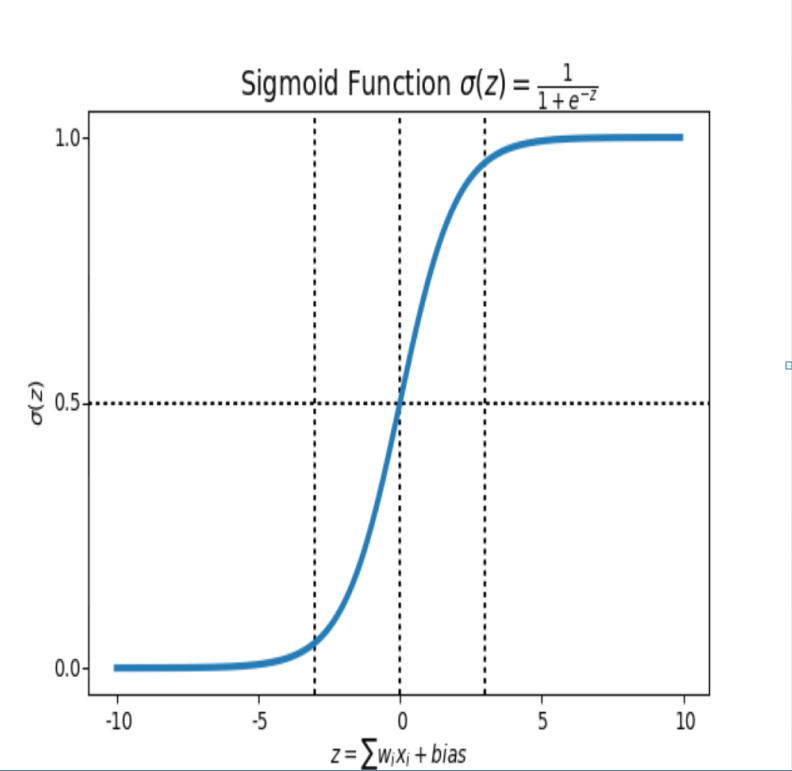
\includegraphics[width=12cm, height=5 cm]{figures/Sigmoid}



\begin{enumerate}
\item When using linear regression we used a formula of the hypothesis i.e.
\begin{itemize}
\item $h{\theta(x)} = \beta_ {0}  + \beta_{1} X$
\end{itemize}
\item For logistic regression we are going to modify it a little bit i.e.
\begin {itemize}
\item $\sigma(Z) = \sigma(\beta_{0} +\beta_{1}X)$
\end{itemize}

\item We have expected that our hypothesis will give values between 0 and 1.
\begin{itemize}

\item $h{\theta(x)} = sigmoid(Z)$
\item $h{\theta(x)} = \frac {1}{1 + e ^- { (\beta_{0}+ \beta_{1}X)}}$
\end{itemize}
\end{enumerate}

 \textbf {Advantages of Logistic regression:  }   
\begin{enumerate}
\item Very efficient
\item Doesn’t require too many resources
\item Easy to regularize
\item Easy to implement
\end{enumerate}
\subsection{K-nearest neighbors (KNN) mode}  
KNN is an algorithm that is considered both non-parametric and an example of lazy learning.\cite{towardsdatascience2} 
\begin{itemize}
\item Non-parametric means that it makes no assumptions. The model is made up entirely from the data given to it rather than assuming its structure is normal.
\item Lazy learning means that the algorithm makes no generalizations. This means that there is little training involved when using this method. Because of this, all of the training data is also used in testing when using KNN.
\end{itemize}
 Its classification uses k which is the number of its nearest neighbors , step of implementations :
\begin{itemize}
\item Calculation of the distance between all points
\item Finds the k points that are closest
\item The class is chosen by the majority of the surrounding points.
\end{itemize}





\section{Project Schedule}
\begin{table}[H]
\centering % used for centering table
\begin{tabular}{c c } % centered columns (4 columns)
\hline\hline %inserts double horizontal lines
Target & Deadline \\ [0.5ex] % inserts table
%heading
\hline % inserts single horizontal line
Data Pre-proccesing & 31 October \\ % inserting body of the table
Data visualization & 7 November \\
Learning Naive Bayes method & 14 November  \\
Learning KNN and logistics regression methods   & 21 November \\
Submitting Prototype & 25 November \\
Final submission & 15 December \\ [1ex] % [1ex] adds vertical space
\hline %inserts single line
\end{tabular}
\label{table:nonlin} % is used to refer this table in the text
\end{table}
\vfil


\section{Personal Websites}
\begin{enumerate}
\item \href{https://asmaamahmoud12.github.io/Asmaa-Mahmoud/}{Asmaa Mahmoud}
\item \href{https://alaagamal98.github.io/}{Alaa Gamal}
\item \href{https://salmazakariia.github.io/SalmaZakaria/}{Salma Zakaria}
\item \href{https://marwaayosiif.github.io/MarwaYoussif/}{Marwa Adel}
\end{enumerate}


\newpage
 \begin{thebibliography}{10}


\bibitem{encyclopedia} 
Thoracic Surgery | Encyclopedia.com
\\\texttt{\url{http://bit.ly/2BTPxzL}}
\bibitem{towardsdatascience1} 
The Actual Difference Between Statistics and Machine Learning
\\\texttt{\url{http://bit.ly/2PloPI2}}
\bibitem{archive} 
UCI Machine Learning Repository: Thoracic Surgery Data Data Set
\\\texttt{\url{http://bit.ly/2MNVjsW}}
\bibitem{researchgate} 
(PDF) Analyzing and visualizing Thoracic Surgery Data Set
\\\texttt{\url{http://bit.ly/364giit}}
\bibitem{analyticsvidhya1} 
A Simple Introduction to ANOVA (with applications in Excel)
\\\texttt{\url{http://bit.ly/2Wdmj7Y}}
\bibitem{mathsisfun} 
Chi-Square Test
\\\texttt{\url{http://bit.ly/2MP5TzT}}
\bibitem{datacamp} 
Introduction to Data Visualization with ggplot2 | DataCamp
\\\texttt{\url{http://bit.ly/2qKiYlo}}
\bibitem{analyticsvidhya2} 
6 Easy Steps to Learn Naive Bayes Algorithm 
\\\texttt{\url{http://bit.ly/2MKPqMN}}
\bibitem{machinelearningmastery} 
Logistic Regression for Machine Learning
\\\texttt{\url{http://bit.ly/2NahU1H}}
\bibitem{towardsdatascience2} 
Machine Learning Basics with the K-Nearest Neighbors Algorithm
\\\texttt{\url{http://bit.ly/367NENp}}

\end{thebibliography}
\end{document}



